\documentclass[10pt]{article}
\usepackage[left=0.9in,top=0.9in,bottom=0.9in,right=0.9in]{geometry}
\usepackage[english]{babel}
\usepackage{fancyhdr}
\usepackage{lastpage}
\usepackage{caption}
\usepackage{amsmath}
\usepackage{hyperref}
\usepackage{xcolor}
\usepackage{graphicx}
\usepackage{float}
\usepackage{textcomp}
\usepackage{amssymb}
\usepackage{mathrsfs}
\usepackage{soul}
\usepackage{enumerate}
\usepackage{wrapfig}
\usepackage{listings}


% Listings settings
\lstset{frame=tb,
  language=Python,
  aboveskip=3mm,
  belowskip=3mm,
  showstringspaces=false,
  columns=flexible,
  basicstyle={\scriptsize\ttfamily},
  breaklines=true,
  breakatwhitespace=true,
  tabsize=3,
  numbers=left,
  xleftmargin=4em,
  framexleftmargin=3.5em
}

% Remove bibliography title
\usepackage{etoolbox}
\patchcmd{\thebibliography}{\section*{\refname}}{}{}{}

% Set up header/footers
\pagestyle{fancy}
\fancyhead[LE,RO]{\today}
\fancyhead[C]{NE 255 - HW 3}
\fancyhead[LO,RE]{D. Hellfeld}
\fancyfoot[C]{\thepage\ of \pageref{LastPage}}
\renewcommand{\headrulewidth}{0.4pt}
\renewcommand{\footrulewidth}{0.4pt}

% Set up figure/table captions
\addto\captionsenglish{\renewcommand{\figurename}{Fig.}}
\addto\captionsenglish{\renewcommand{\tablename}{\small Table}}
\renewcommand{\thetable}{\Roman{table}}
\captionsetup[table]{labelfont = normal, labelsep=period, singlelinecheck=false}
\captionsetup[figure]{labelfont=normal, labelsep=period, singlelinecheck=false}

% Remove paragraph indent
\setlength\parindent{0pt}


\begin{document}


% - - - - - - - - - - - - - - - - - - - - - - - - - - - - - - - - - - - - - - - - - -
\begin{centering}
\textbf{\large NE 255 - Homework 3}\\
\vspace{11pt}
University of California, Berkeley\\
Department of Nuclear Engineering\\
\vspace{11pt}
Daniel Hellfeld\\
\href{mailto:dhellfeld@berkeley.edu}{dhellfeld@berkeley.edu}\\
\end{centering}




% - - - - - - - - - - - - - - - - - - - - - - - - - - - - - - - - - - - - - - - - - -
\vspace{22pt}
\noindent \textbf{Problem 1}\\
Derive the 1\textsuperscript{st} order form of SP$_5$ with isotropic source and vacuum boundary conditions. \\[5pt]


$\Rightarrow$ We begin by considering the slab geometry P$_N$ equations derived in class
%
\begin{equation*}
    \left(\frac{l'+1}{2l'+1}\right)\frac{d}{d x}\phi_{l'+1}(x) + \left(\frac{l'}{2l'+1}\right)\frac{d}{d x}\phi_{l'-1}(x) + \Sigma_t(x) \phi_{l'} = \Sigma_{sl'}(x)\phi_{l'}(x) + s_{l'}(x)\:,
\end{equation*}

for $l' = 0, 1, ... , N$. We also set $\phi_{-1}=0$ and $\phi_{N+1} = 0$ or ($\frac{d}{dx}\phi_{N+1}=0$). Now to \emph{heuristically} derive the SP$_N$ equations, we use Gelbard's idea of making simple substitutions to put us into a 3D system (we could use an asymptotic analysis to derive SP$_N$, but the heuristic approach is much simpler). To do so, we first replace odd $l'$ values of $\phi_{l'}$ with a vector:
%
\begin{equation*}
    \phi_{l'} \rightarrow \vec{\phi}_{l'} = (\phi_{l'}^x,\phi_{l'}^y,\phi_{l'}^z)^t\,.
\end{equation*}

Then, for even $l'$ equations, the space derivative becomes a divergence:
%
\begin{equation*}
    \frac{d}{dx} \rightarrow \nabla \cdot\,\,,
\end{equation*}

and for the odd $l'$ equations the space derivative becomes a gradient:
%
\begin{equation*}
    \frac{d}{dx} \rightarrow \nabla\,\,.
\end{equation*}

Making these substitutions into the P$_N$ equations above and separating into $l'=0$, $l'$ even, and $l'$ odd equations, we arrive at the first-order form of the SP$_N$ equations
%
\begin{align*}
    &\nabla \cdot \vec{\phi}_1 + \Sigma_a \phi_0 = s_0, \hspace{255pt}(l'=0)\\
    &\Big(\frac{l'+1}{2l'+1}\Big) \nabla\phi_{l'+1} + \Big(\frac{l'}{2l'+1}\Big)\nabla\phi_{l'-1} + \Sigma_t \vec{\phi}_{l'} = \Sigma_{sl'} \vec{\phi}_{l'} + s_{l'}, \hspace{80pt}(l'\textrm{ odd})\\
    &\Big(\frac{l'+1}{2l'+1}\Big) \nabla \cdot \vec{\phi}_{l'+1} + \Big(\frac{l'}{2l'+1}\Big)\nabla\cdot\vec{\phi}_{l'-1} + \Sigma_t \phi_{l'} = \Sigma_{sl'} \phi_{l'} + s_{l'}, \hspace{30pt}(l'\textrm{ even},\,\,l'>0)
\end{align*}

where $l'=0,1,2, ... , N$, $\phi$ is the three-dimensional scalar flux, $\phi_{l'}$ is the ${l'}$\textsuperscript{th} moment of the scalar flux, $\vec{\phi}_{l'} = (\phi_{l'}^x,\phi_{l'}^y,\phi_{l'}^z)^T$ (for odd $l'$), $\Sigma_t$ is the total interaction cross-section, $\Sigma_{sl'}$ is the ${l'}$\textsuperscript{th} moment scattering cross-section, and $s_{l'}$ is the ${l'}$\textsuperscript{th} moment of an arbitrary neutron source (which could include fission). I did not include space dependences in the equations as to avoid clutter, but the scalar flux, cross-sections, and source will have spatial ($x,y,z$) dependencies.\\

Plugging in for $N=5$, we arrive at the following six equations
%
\begin{align*}
    &l'=0\ \ \ \Rightarrow\ \ \ \nabla \cdot \vec{\phi}_1 + \Sigma_a \phi_0 = s_0\\
    &l'=1\ \ \ \Rightarrow\ \ \ \Big(\frac{2}{3}\Big) \nabla\phi_{2} + \Big(\frac{1}{3}\Big)\nabla\phi_{0} + \Sigma_t \vec{\phi}_{1} = \Sigma_{s1} \vec{\phi}_{1} + s_{1}\\
    &l'=2\ \ \ \Rightarrow\ \ \ \Big(\frac{3}{5}\Big) \nabla \cdot \vec{\phi}_{3} + \Big(\frac{2}{5}\Big)\nabla\cdot\vec{\phi}_{1} + \Sigma_t \phi_{2} = \Sigma_{s2} \phi_{2} + s_{2} \\
    &l'=3\ \ \ \Rightarrow\ \ \ \Big(\frac{4}{7}\Big) \nabla\phi_{4} + \Big(\frac{3}{7}\Big)\nabla\phi_{2} + \Sigma_t \vec{\phi}_{3} = \Sigma_{s3} \vec{\phi}_{3} + s_{3} \\
    &l'=4\ \ \ \Rightarrow\ \ \ \Big(\frac{5}{9}\Big) \nabla \cdot \vec{\phi}_{5} + \Big(\frac{4}{9}\Big)\nabla\cdot\vec{\phi}_{3} + \Sigma_t \phi_{4} = \Sigma_{s4} \phi_{4} + s_{4} \\
    &l'=5\ \ \ \Rightarrow\ \ \ \Big(\frac{6}{11}\Big) \nabla\phi_{6} + \Big(\frac{5}{11}\Big)\nabla\phi_{4} + \Sigma_t \vec{\phi}_{5} = \Sigma_{s5} \vec{\phi}_{5} + s_{5}
\end{align*}

In the SP$_N$ approximation, we set $\phi_{N+1}=0$ or equivalently $\nabla\phi_{N+1}=0$, therefore $\nabla \phi_6 = 0$. With an isotropic source, we can set all $l'\geq1$ moments of the source to 0 ($s_1= s_2=s_3=s_4=s_5=0$):
%
\begin{align*}
    &l'=0\ \ \ \Rightarrow\ \ \ \nabla \cdot \vec{\phi}_1 + \Sigma_a \phi_0 = s_0\\
    &l'=1\ \ \ \Rightarrow\ \ \ \Big(\frac{2}{3}\Big) \nabla\phi_{2} + \Big(\frac{1}{3}\Big)\nabla\phi_{0} + (\Sigma_t - \Sigma_{s1}) \vec{\phi}_{1} = 0\\
    &l'=2\ \ \ \Rightarrow\ \ \ \Big(\frac{3}{5}\Big) \nabla \cdot \vec{\phi}_{3} + \Big(\frac{2}{5}\Big)\nabla\cdot\vec{\phi}_{1} + (\Sigma_t - \Sigma_{s2}) \phi_{2} = 0 \\
    &l'=3\ \ \ \Rightarrow\ \ \ \Big(\frac{4}{7}\Big) \nabla\phi_{4} + \Big(\frac{3}{7}\Big)\nabla\phi_{2} + (\Sigma_t - \Sigma_{s3}) \vec{\phi}_{3} = 0 \\
    &l'=4\ \ \ \Rightarrow\ \ \ \Big(\frac{5}{9}\Big) \nabla \cdot \vec{\phi}_{5} + \Big(\frac{4}{9}\Big)\nabla\cdot\vec{\phi}_{3} + (\Sigma_t -\Sigma_{s4}) \phi_{4} = 0\\
    &l'=5\ \ \ \Rightarrow\ \ \ \Big(\frac{5}{11}\Big)\nabla\phi_{4} + (\Sigma_t-\Sigma_{s5}) \vec{\phi}_{5} = 0
\end{align*}

We could relate some of the $\phi$'s to each other and reduce these equations to get to the \emph{second order form}, but we will stop here.\\

The vacuum boundary conditions in the SP$_N$ equations are obtained for all $\phi_{l'}$ by replacing $\mu$ with $\vec{n} \cdot \hat{\Omega}$ in the P$_N$ Marshak vacuum boundary conditions, where $\vec{n}$ is the inward-normal and $\hat{\Omega}$ describes the direction of the flux. The P$_N$ Marshak vacuum boundary conditions are given by
%
\begin{align*}
    \int_{\mu_{in}} d\mu P_l(\mu)\psi(\vec{r}_0,\mu) = 0,\ \ \textrm{  for odd $l$ }(=1,3,5,...,N)
\end{align*}

where $P_l(\mu)$ are the Legendre polynomials and $\vec{r}_0$ is the position of the boundary. Expanding the angular flux in Legendre polynomials, we arrive at
%
\begin{align*}
    \int_{\mu_{in}} d\mu P_l(\mu)\sum_{n=0}^{\infty}\Big(\frac{2n+1}{4\pi}\Big) \phi_n(\vec{r}_0)P_n(\mu) = 0,\ \ \textrm{  for odd $l$ }(=1,3,5,...,N)
\end{align*}

and pulling out some terms from the integral
%
\begin{align*}
    \Rightarrow\,\, \sum_{n=0}^{\infty}\Big(\frac{2n+1}{4\pi}\Big) \phi_n(\vec{r}_0)\int_{\mu_{in}} d\mu P_l(\mu)P_n(\mu) = 0,\ \ \textrm{  for odd $l$ }(=1,3,5,...,N)
\end{align*}


Now, we replace the $\mu$'s with $\vec{n}\cdot \hat{\Omega}$, the integral over the inward coming $\mu$'s becomes an integral over $\hat{\Omega}$ where $\vec{n}\cdot \hat{\Omega} > 0$ (which is to say the inward coming flux), and finally we replace the $\phi_n$'s with our even and odd $\phi$'s from the SP$_N$ equations (I will now use $n$ instead of $l'$ as to not get confused with $l$). When we separate out the even and odd $\phi$'s, we will have two terms and we will have to dot the odd $\phi$'s (vector) with the inward normal vector ($\vec{n}$). Doing all this, we arrive at
%
\begin{align*}
    \sum_{n\textrm{ even}}\Big(\frac{2n+1}{4\pi}\Big) &\phi_n(\vec{r}_0) \int_{\vec{n}\cdot \hat{\Omega} > 0} d\hat{\Omega} P_l(\vec{n}\cdot \hat{\Omega})P_n(\vec{n}\cdot \hat{\Omega}) \ \ + \\
    & \sum_{n\textrm{ odd}}\Big(\frac{2n+1}{4\pi}\Big) \vec{n} \cdot \vec{\phi}_n(\vec{r}_0) \int_{\vec{n}\cdot \hat{\Omega} > 0} d\hat{\Omega} P_l(\vec{n}\cdot \hat{\Omega})P_n(\vec{n}\cdot \hat{\Omega}) = 0,\ \ \ \ \textrm{  for odd $l$ }(=1,3,5,...,N)
\end{align*}

Now if we were integrating over the whole range, we would be able to use the orthogonality of Legendre polynomials to cancel out the even terms (because $l$ is only defined to be odd), but this is not the case.








% - - - - - - - - - - - - - - - - - - - - - - - - - - - - - - - - - - - - - - - - - -
\newpage
\noindent \textbf{Problem 2}\\
Consider the integral
%
\begin{equation*}
\int_{4\pi} d\hat{\Omega}\,\hat{\Omega}
\end{equation*}

The LQ$_N$ quadrature set is given in Table 4-1 in Lewis and Miller (\emph{E.E.~Lewis and W.F.~Miller, Computational Methods of Neutron Transport, John Wiley \& Sons, Inc., 1984.}). Recall that $\mu_i = \eta_i= \xi_i$ for a given level, $i$.
%
\begin{enumerate}[(a)]
\item Use the S$_4$ LQ$_N$ quadrature set to execute this integral.\\[-5pt]
\end{enumerate}

$\Rightarrow$ A quadrature set allows us to evaluate the integral of a function over some domain using a discrete set of points and corresponding weights:
%
\begin{equation*}
    \int dx f(x) = \sum_{n \in \textrm{set}} w_n f(n)
\end{equation*}

Now, we can decompose $\hat{\Omega}$ into its directional cosines ($\mu$, $\eta$, and $\xi$) like $\hat{\Omega} = \sqrt{\mu^2 + \eta^2 + \xi^2}$ (= 1) and use the LQ$_N$ quadrature set to determine the weights at each $\mu_i$, $\eta_i$, and $\xi_i$, where at each level $\mu_i = \eta_i = \xi_i$. In each S$_N$ set, we have $N(N+2)/8$ quadrature points in each octant, therefore for S$_4$ we have 3 points which, using Fig.\,1a below, correspond to \{$\mu_1, \eta_1, \xi_2$\}, \{$\mu_1, \eta_2, \xi_1$\}, and \{$\mu_2, \eta_1, \xi_1$\}. Using Table 4-1, we have that $\mu_1 = \eta_1 = \xi_1 = 0.3500212$ with a weight of 0.3333333 and $\mu_2 = \eta_2 = \xi_2 = 0.8688903$ also with a weight of 0.3333333. Plugging all this in, we get
%
\begin{equation*}
    \int_{4\pi} d\hat{\Omega}\,\hat{\Omega} \approx \sum_{\textrm{8 octants}} w\sqrt{\mu_1^2 + \eta_1^2 + \xi_2^2} + w\sqrt{\mu_1^2 + \eta_2^2 + \xi_1^2} + w\sqrt{\mu_2^2 + \eta_1^2 + \xi_1^2}
\end{equation*}

Since all the directional cosines are squared in the equation for $\hat{\Omega}$, we do not need to care much about the fact that they can be negative in certain octants (\ul{however in general we would have to be careful about signs}). Therefore the sum over the 8 octants can be reduced to just multiplying by 8.
%
\begin{align*}
        \int_{4\pi} d\hat{\Omega}\,\hat{\Omega} &\approx 8 \Big( w\sqrt{\mu_1^2 + \eta_2^2 + \xi_2^2} + w\sqrt{\mu_2^2 + \eta_2^2 + \xi_1^2} + w\sqrt{\mu_2^2 + \eta_1^2 + \xi_2^2} \Big) \\
        &\approx 8 \Big( 0.3333333\sqrt{1} + 0.3333333\sqrt{1} + 0.3333333\sqrt{1} \Big) \\
        &\approx 8 (0.9999999)
\end{align*}

Now, the weights are normalized to 1 in each quadrant and thus 8 over the entire sphere. However, we know that the integral over the sphere should be equal to 4$\pi$. Therefore we have to multiply by a factor of $4\pi /8$ to get the correct answer. Doing so, we get
%
\begin{equation*}
    (4\pi/8)(8)(0.9999999) = (4\pi)(0.9999999)
\end{equation*}

\begin{figure}[H]
    \centering
    \begin{tabular}{cc}
        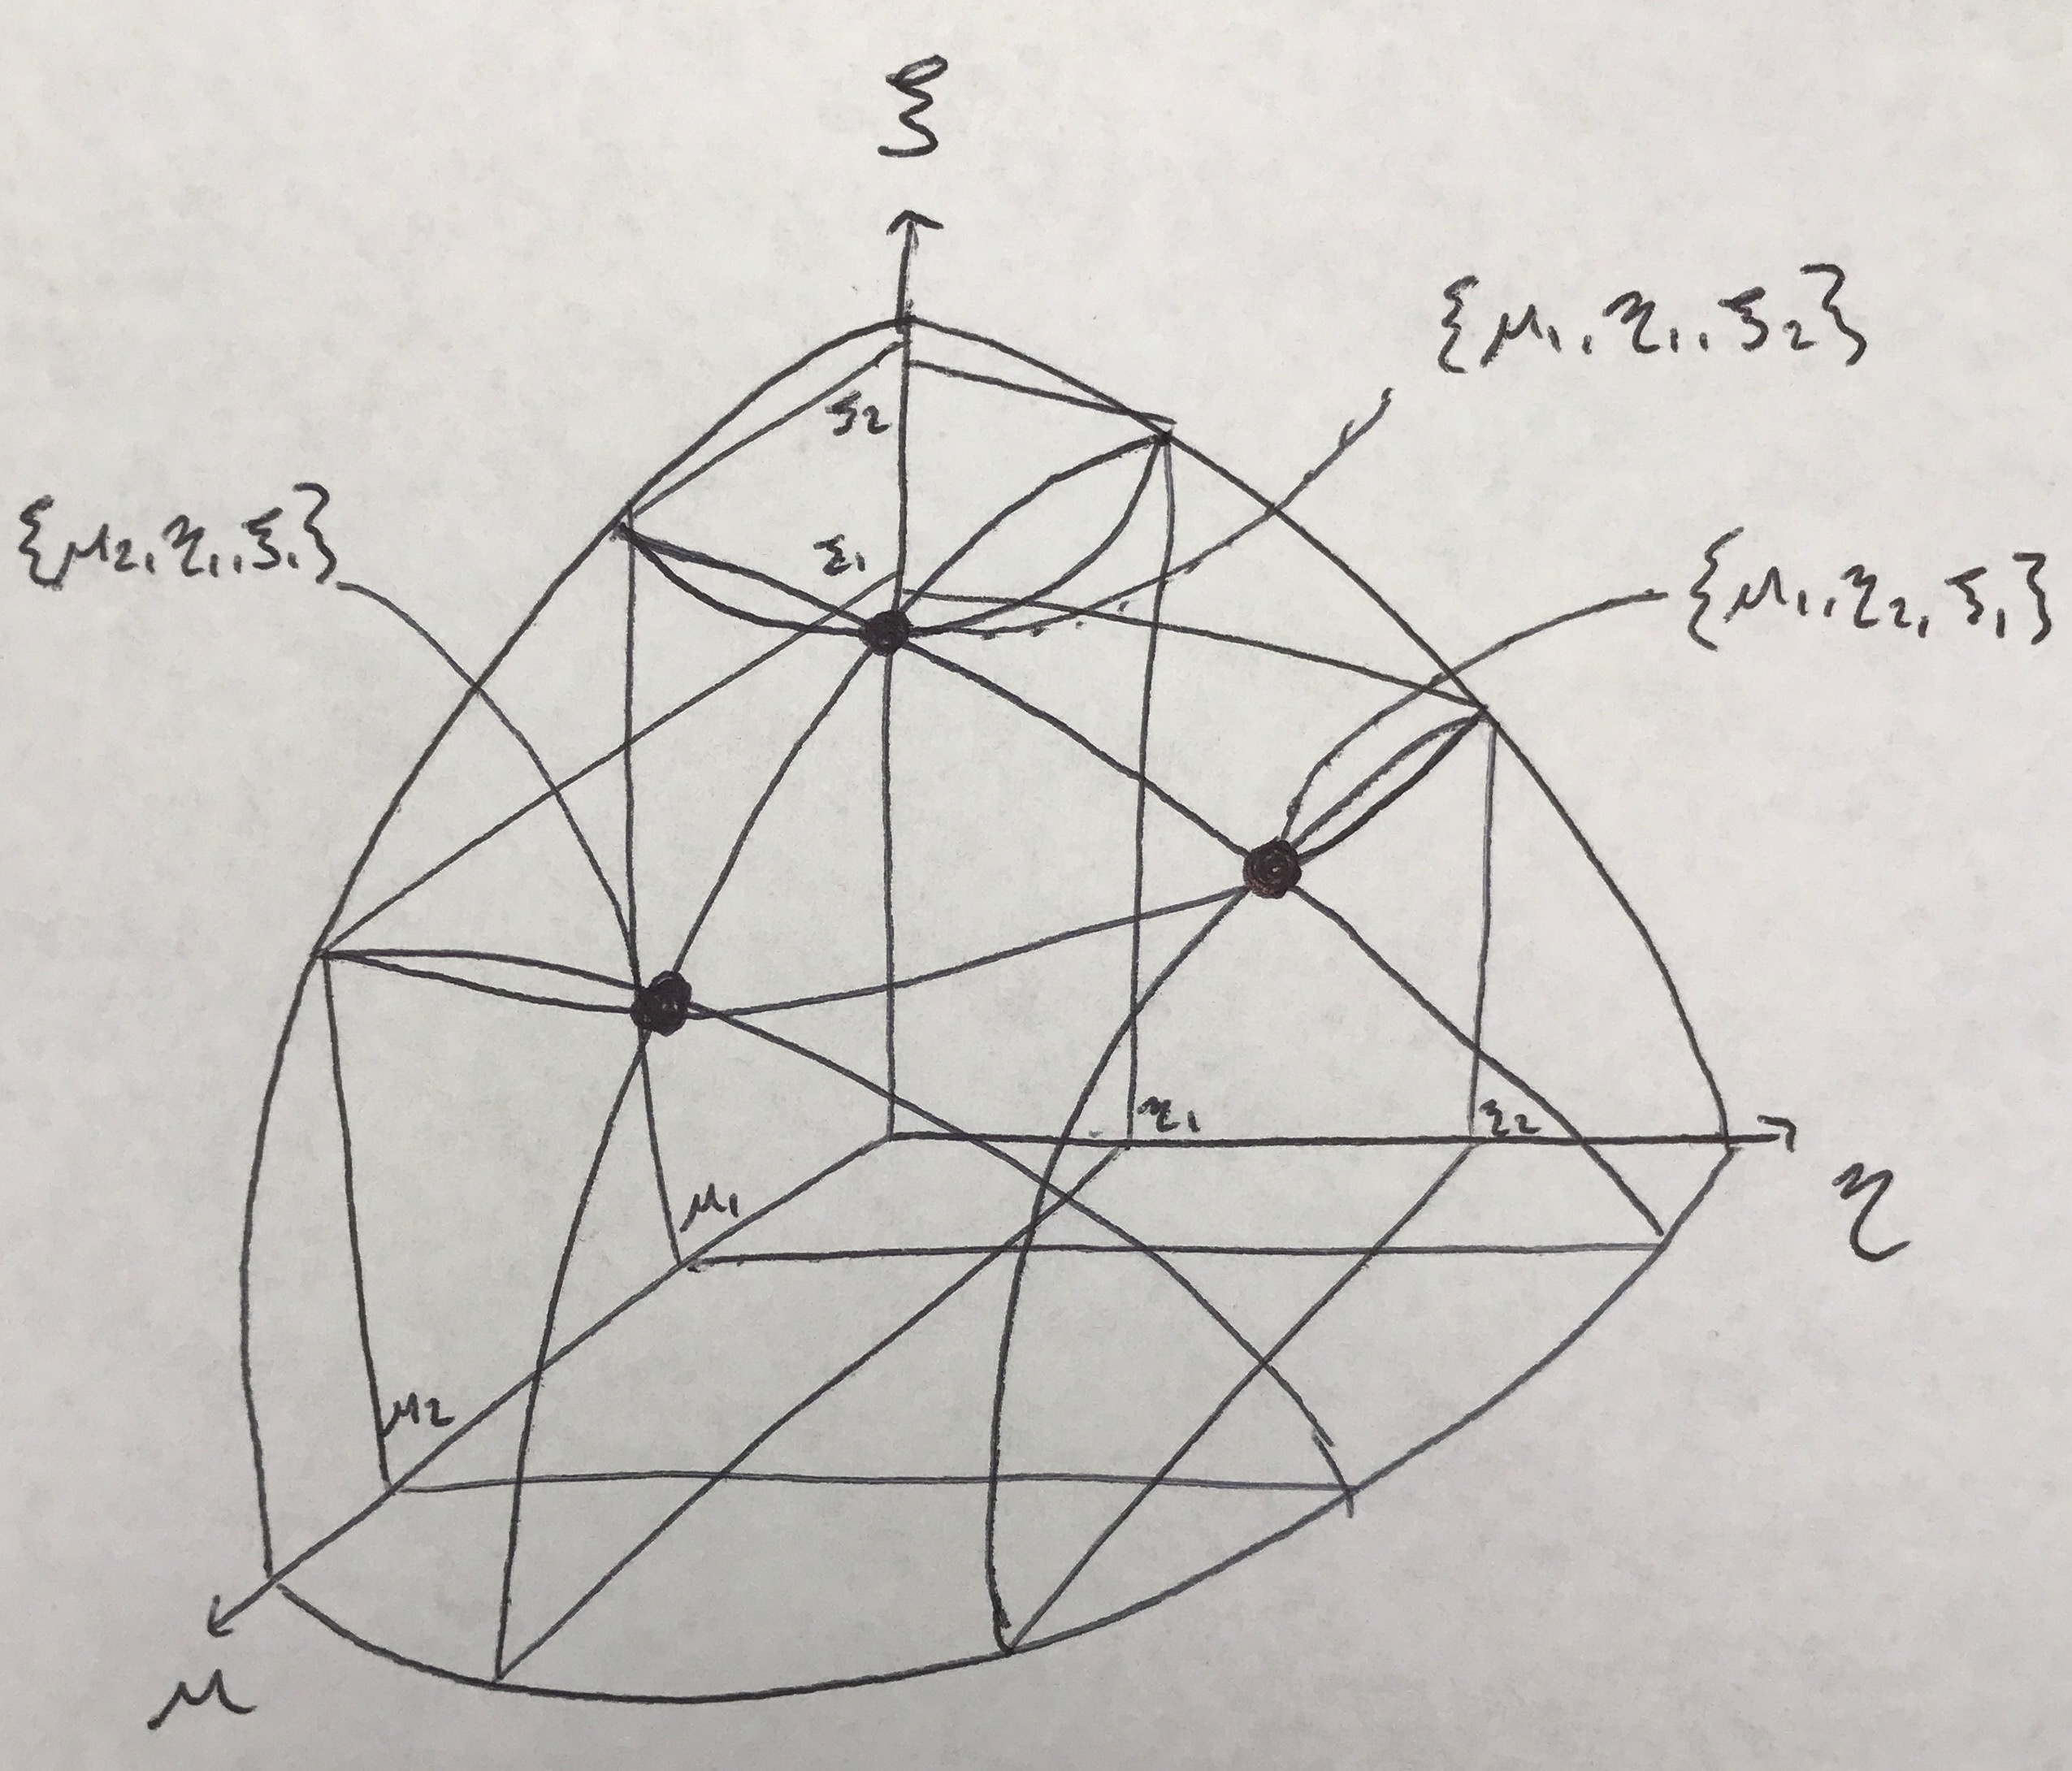
\includegraphics[height=120pt]{Figures/S4.jpg} &
        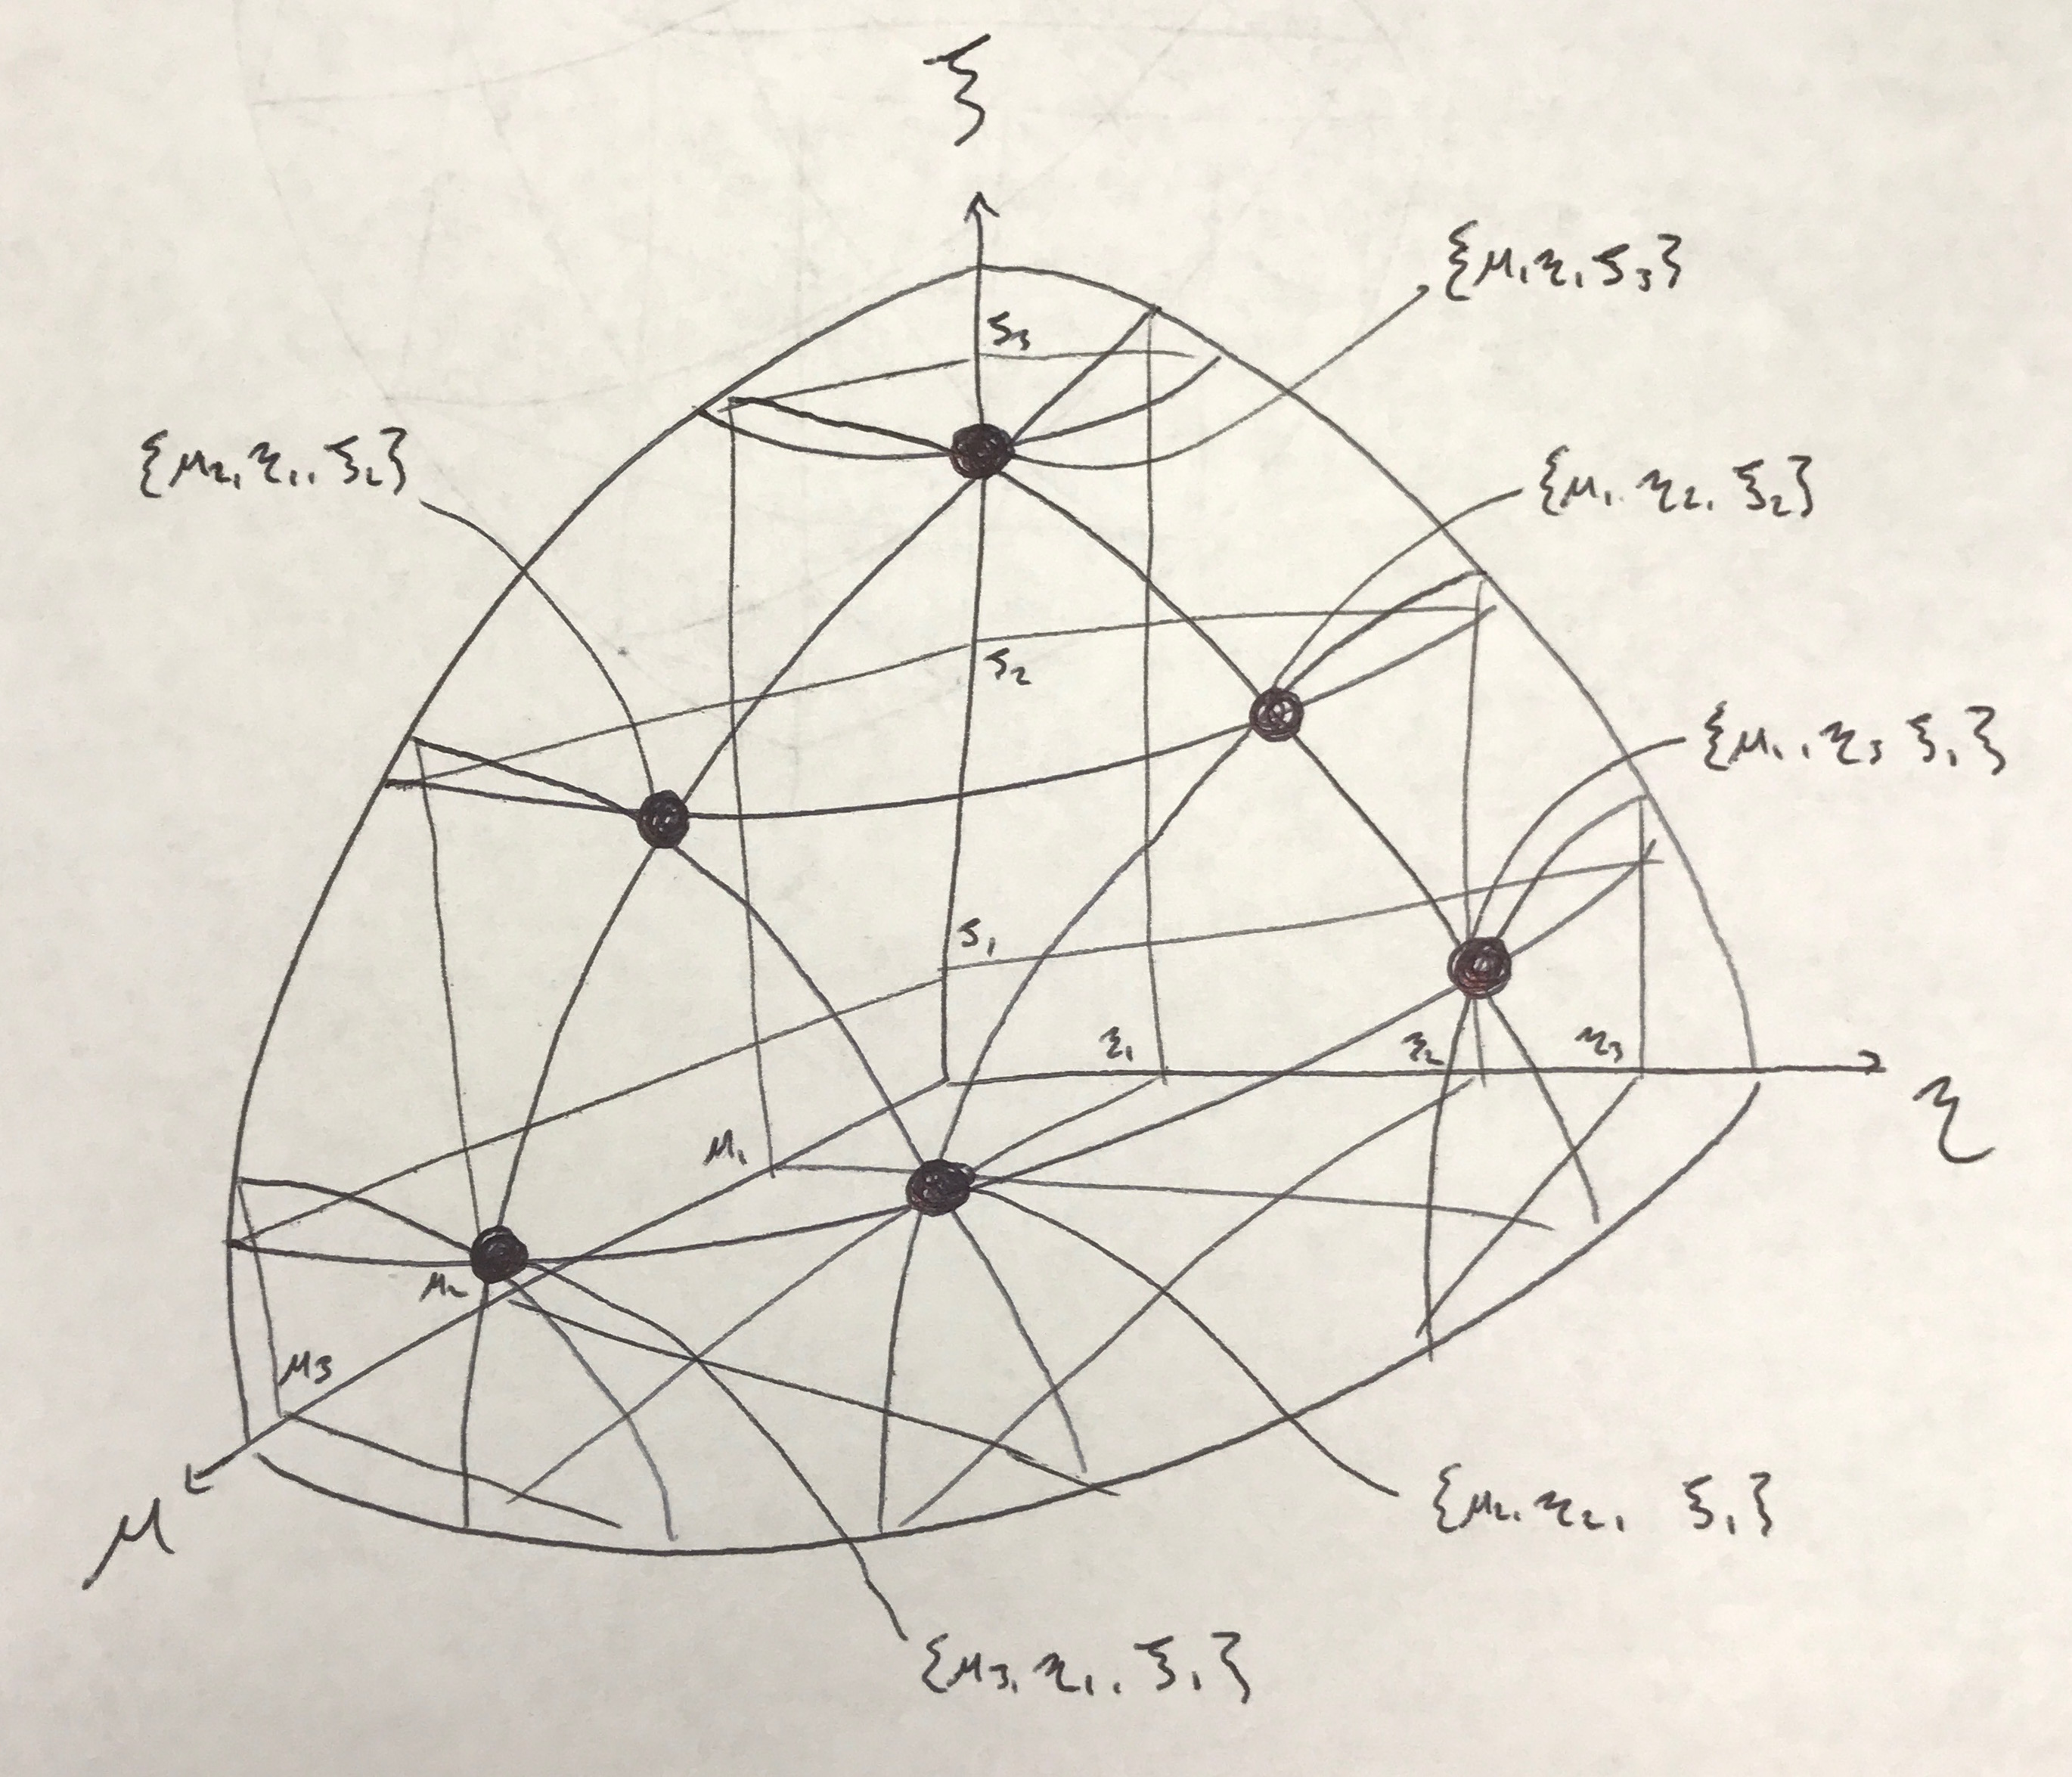
\includegraphics[height=120pt]{Figures/S6.jpg} \\
        \scriptsize{(a)} & \scriptsize{(b)} \\ [-1.2ex]
    \end{tabular}
    \caption{S4 (a) and S6 (b) quadrature point sketches. Please excuse my terrible drawing abilities.}
    \label{fig1}
\end{figure}


\vspace{10pt}
\begin{enumerate}[(b)]
\item Repeat it with S$_6$. What do you observe?\\[-5pt]
\end{enumerate}

$\Rightarrow$ Using S$_6$, we will have the following 6 points (see Fig.\,1b): \{$\mu_1, \eta_1, \xi_3$\}, \{$\mu_3, \eta_1, \xi_1$\}, and \{$\mu_1, \eta_3, \xi_1$\} with weight 0.1761263, and \{$\mu_2, \eta_1, \xi_2$\}, \{$\mu_1, \eta_2, \xi_2$\}, and \{$\mu_2, \eta_2, \xi_1$\} with weight 0.1572071. Plugging in everything, we get
%
\begin{align*}
        \int_{4\pi} d\hat{\Omega}\,\hat{\Omega} \approx (4\pi/8) \sum_{\textrm{8 octants}} \Big( &w_1\sqrt{\mu_1^2 + \eta_1^2 + \xi_3^2} + w_1\sqrt{\mu_3^2 + \eta_1^2 + \xi_1^2} + w_1\sqrt{\mu_1^2 + \eta_3^2 + \xi_1^2} \ + \\
        &w_2\sqrt{\mu_2^2 + \eta_1^2 + \xi_2^2} + w_2\sqrt{\mu_1^2 + \eta_2^2 + \xi_2^2} + w_2\sqrt{\mu_2^2 + \eta_2^2 + \xi_1^2} \Big)
\end{align*}
%
\begin{align*}
        &\Rightarrow (4\pi/8)(8)\Big((3)(0.1761263) + (3)(0.1572071)\Big) \\
        &= (4\pi)(1.0000002)
\end{align*}

We see that this slightly overshoots the true value, by an amount slightly above the value we undershot using S$_4$. But in essence we calculate the same value, as expected.


\vspace{10pt}
\begin{enumerate}[(c)]
\item Write a short code to execute this integration (and higher orders if you'd like). Try a few different functions. Turn in the code and the evaluation of these functions. Include comments on what you observe. \\[-5pt]
\end{enumerate}

$\Rightarrow$ See the Python code below for the quadrature integration of three functions ($f(\hat{\Omega}) = \hat{\Omega}$, $f(\hat{\Omega}) = \mu + \eta + \xi$, and $f(\hat{\Omega}) = \mu^2 = \cos^2(\theta)$) with the ability to use N = 2, 4, 6, 8, 12, and 16.\\

\lstinputlisting[language=Python]{../p2/p2c.py}

Now, we expect the following results for the functions in the script (I do not feel the need to explicitly show the steps)
%
\begin{align*}
    \int_{4\pi} \hat{\Omega}\,d\hat{\Omega} =  4\pi ;\quad\quad
    \int_{4\pi} (\mu + \eta + \xi)\,d\hat{\Omega} = 0 ;\quad\quad
    \int_{4\pi} \mu^2\,d\hat{\Omega} = \int_{4\pi} \cos^2\theta\,d\hat{\Omega} = 2\pi(2/3)
\end{align*}

And if we run the script above for multiple values of N, we get the following results

\begin{table}[htb]
    \centering
    \begin{tabular}{|c|c|c|c|}
        \hline
        & $f(\hat{\Omega}) = \hat{\Omega}$ & $f(\hat{\Omega}) = \mu + \eta + \xi$ & $f(\hat{\Omega}) = \mu^2 = \cos^2(\theta)$ \\ \hline
        True Value & 12.5663706 & 0.0            & 4.1887902 \\\hline
        N = 2      & 12.5663713 & 0.0            & 4.1887907 \\\hline
        N = 4      & 12.5663696 & -8.7196712e-17 & 4.1887899 \\\hline
        N = 6      & 12.5663718 & -6.1037699e-16 & 4.1887901 \\\hline
        N = 8      & 12.5663695 & 2.8338932e-16  & 4.1887899 \\\hline
        N = 12     & 12.5663730 & -6.6487493e-16 & 4.1887910 \\\hline
        N = 16     & 12.5663619 & 1.2316536e-15  & 4.1887874 \\\hline
    \end{tabular}
\end{table}

All the quadrature sets seem to approximate the integrals fairly well, up to what seems to be most likely just rounding errors. Also notice that is seems to alternate in overshooting and undershooting as $N$ is increased.






% - - - - - - - - - - - - - - - - - - - - - - - - - - - - - - - - - - - - - - - - - -
\newpage
\noindent \textbf{Problem 3}\\ [-4ex]
\begin{enumerate}[(a)]
    \item Briefly compare the diffusion equation, deterministic methods, and Monte Carlo methods in terms of complexity, accuracy, run time, and range of applicability. \\[-5pt]
\end{enumerate}

$\Rightarrow$ The diffusion equation is an approximation to the transport equation - specifically under the assumptions of azimuthally symmetric scattering, scattering is at most linear anisotropic, and that the angular flux is also at most linearly anisotropic. Solutions are not valid when solved for near voids, boundaries, sources, or in strongly absorbing media. This severely limits the applicability of the diffusion equation, but for most macroscopic quantities we are concerned about in nuclear reactor physics (such as nuclear interaction rates, i.e.\,\,fission) this can be acceptable. The diffusion equation is quite simple and can in some cases be solved analytically by hand or using simple diffusion solvers.\\

Deterministic methods are methods by which we try to solve the transport or diffusion equation. This is done by discretizing all the variables in the equation (including time, space, energy, and direction), solving equations in each discretized space, and correctly communicating information between the discretized spaces. The complexity, accuracy, and run time are all dependent on the extent of discretization. If finer discretization is used, the solutions are more accurate, but the equations become more complex and the computational expenses significantly increase. While the equations in the solvers can be complex, the inputs given to the solvers tend to be quite simple (I want this solution in this system using these discretizations, etc.). Deterministic solutions are also global in the sense that the solutions we produce are valid in the entire space (constrained by the meshing, of course). \\

Monte Carlo methods are akin to deterministic methods as they are both methods to solve the diffusion or transport equation. In contrast to deterministic methods, however, in Monte Carlo we use continuous variables and sample every single interaction every particle has until we have sampled enough times that the solution we generate is statistically significant. We therefore do not necessary solve any equations (apart from the interaction probability sampling equations), but instead follow multiple particles through multiple stochastic histories to find an average behavior of some unknown (such as the neutron flux). Monte Carlo is regarded, in most cases, as much less complex than deterministic methods (though correctly sampling interactions can be difficult as well as building the geometry and including all the necessary physics), but it comes at a price of run time. Because so many particle histories need to be run in order to gain sufficient statistics, Monte Carlo methods are typically slower than deterministic. However, Monte Carlo is also much easier to parallelize (because each particle history is independent of the others and thus they can be simulated at the same time) which can lead to significant speed ups. With increased run time, we will get a more precise answer (a smaller uncertainty), however it does not always promise a more accurate answer (that relies on the correct modeling of both the system and the physics). The solutions we generate with Monte Carlo are also considered local solutions (as opposed to deterministic methods) because of the use of local tallies, such as the neutron flux at a specific point in space (as opposed to the flux everywhere). We do this because to generate enough statistics to the get the global solution would take a enormous amount of time!\\




\begin{enumerate}[(b)]
    \item Given what you've learned about deterministic methods so far, discuss strengths and weaknesses.\\[-5pt]
\end{enumerate}

$\Rightarrow$ The strengths of deterministic methods are that they are fast, they produce global solutions that have the same quality everywhere in the solution space, and the inputs to the solvers can be simple. The weaknesses are that the quality of the solutions are dependent on the level of discretization (which can become very computationally intensive, and it remains difficult to parallelize deterministic codes on CPUs) and solutions will always include some truncation error. Also, the solutions we produce are only valid in the meshing we input and we are subject to Ray Effects - if we only solve along certain directions, then in certain cases such as low scattering media, then our solutions are constrained only to the directions we input and the solution space we solve in can become quite sparse.





% - - - - - - - - - - - - - - - - - - - - - - - - - - - - - - - - - - - - - - - - - -
\newpage
\noindent \textbf{Problem 4}\\
Write a function that generates the associated Legendre Polynomials
%
\begin{equation*}
    P_l^m(x) = \frac{(-1)^m}{2^l l!}(1-x^2)^{m/2}\frac{d^{l+m}}{dx^{l+m}}(x^2-1)^l
\end{equation*}

Use this function in a function that generates spherical harmonics

\begin{equation*}
    Y_{lm}(\theta,\varphi)=(-1)^m\sqrt{\frac{2l+1}{4\pi}\frac{(l-m)!}{(l+m)!}}P_{lm}(\cos\theta)e^{-im\varphi}
\end{equation*}

\begin{enumerate}[(a)]
    \item Generate and plot the following $l = 0, 1, 2$ for $−l \leq m \leq l$ (recall we can relate the negative $m$ to positive $m$ values). You will need to discretize $\theta$ and $\mu$ fairly finely (I suggest 30 increments in each to start so you get a real sense of the shape of the harmonics). \\[-5pt]
\end{enumerate}

$\Rightarrow$ See the attached Python script below for the generation of the associated Legendre Polynomials and Spherical Harmonics. The script produces 3D plots using the mayavi package, and 2D screenshots are shown in Fig.~1 for both the real and imaginary parts. In the plots, I use two methods to visualize the spherical harmonics - a heat map on a unit sphere where the color corresponds to the value of the spherical harmonic at a particular $\theta$ and $\phi$, and a distorted sphere where the distance from the origin represents the absolute value of the spherical harmonic at a particular $\theta$ and $\phi$ (the color represents the true value of the spherical harmonic). \\

\lstinputlisting[language=Python]{../p4/a/p4a.py}

\begin{figure}[H]
    \centering
    \begin{tabular}{|c|c|c|c|c|c|}
    \hline
    \textbf{Real} & m = 0 & m = -1 & m = 1 & m = -2 & m = 2 \\ \hline
    l = 0 & 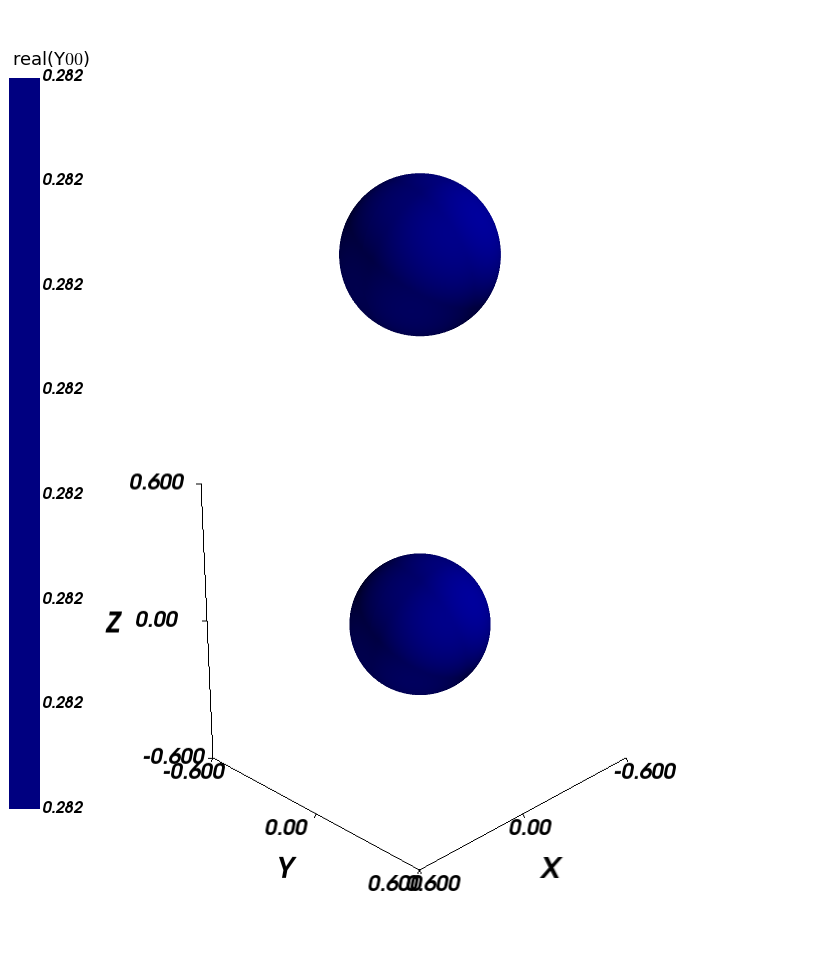
\includegraphics[height=0.17\textwidth]{Figures/y00.png} &&&& \\ \hline
    l = 1 & 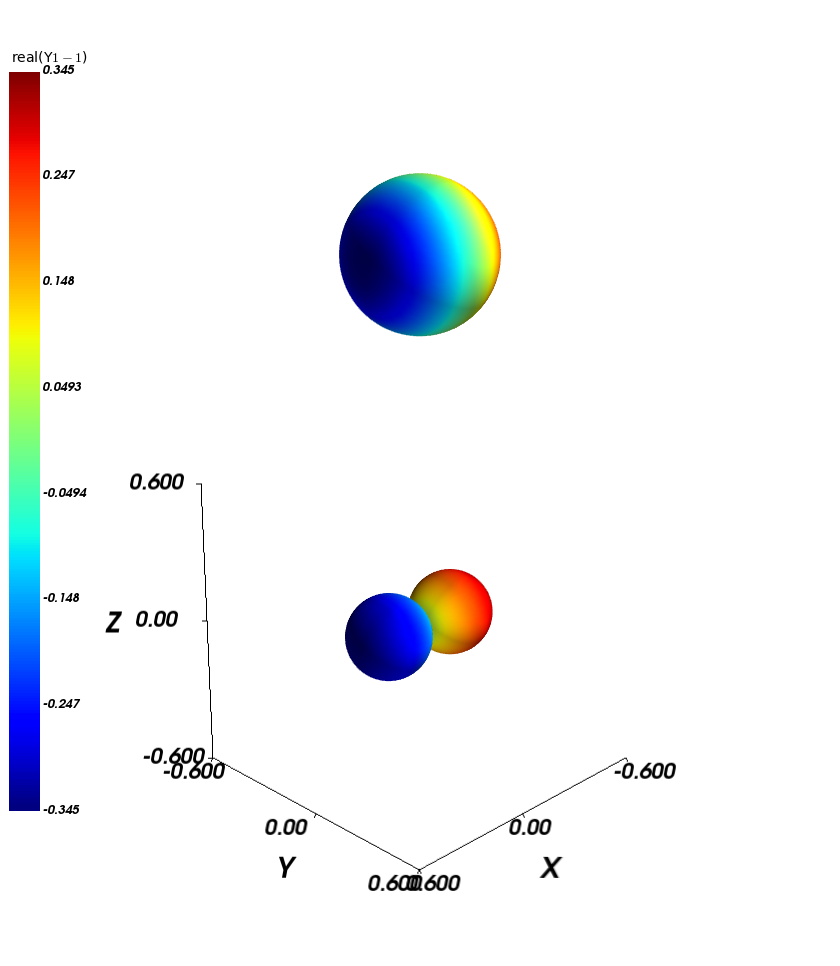
\includegraphics[height=0.17\textwidth]{Figures/y1-1.png} &
    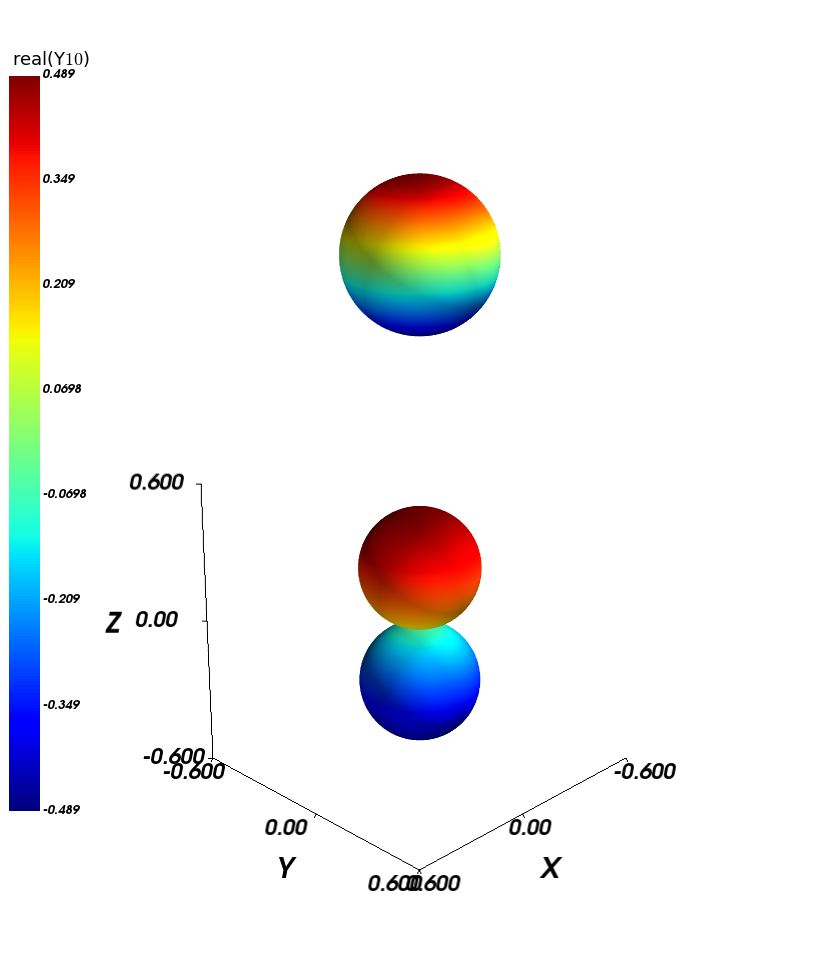
\includegraphics[height=0.17\textwidth]{Figures/y10.png} &
    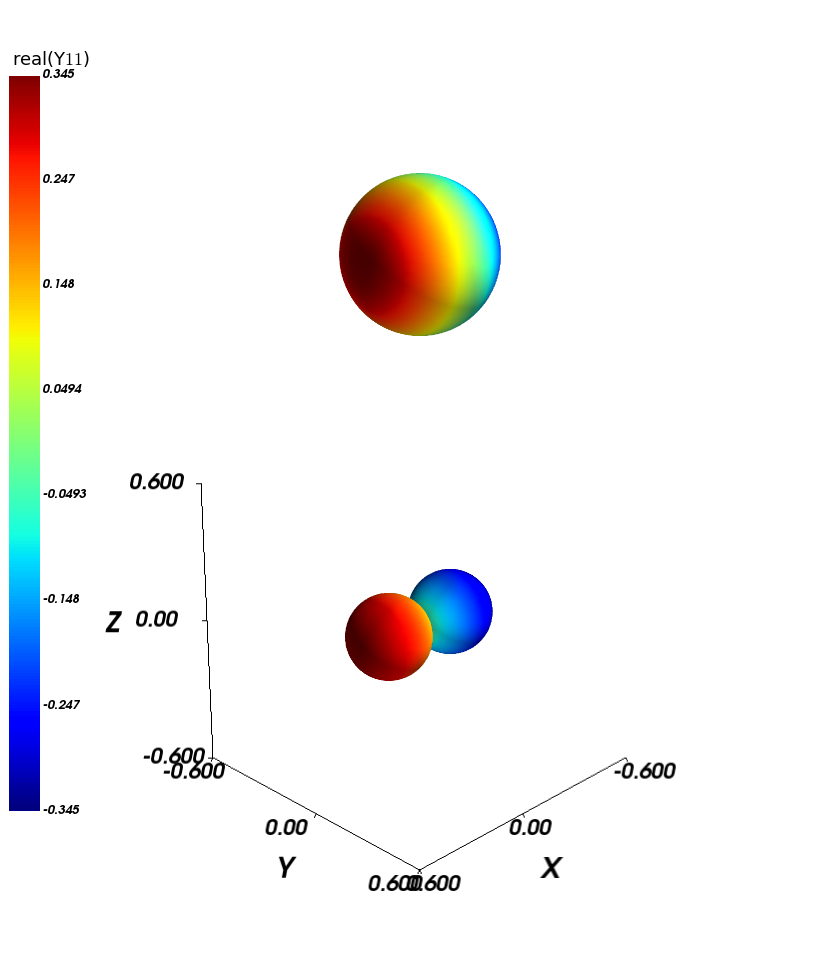
\includegraphics[height=0.17\textwidth]{Figures/y11.png} && \\ \hline
    l = 2 & 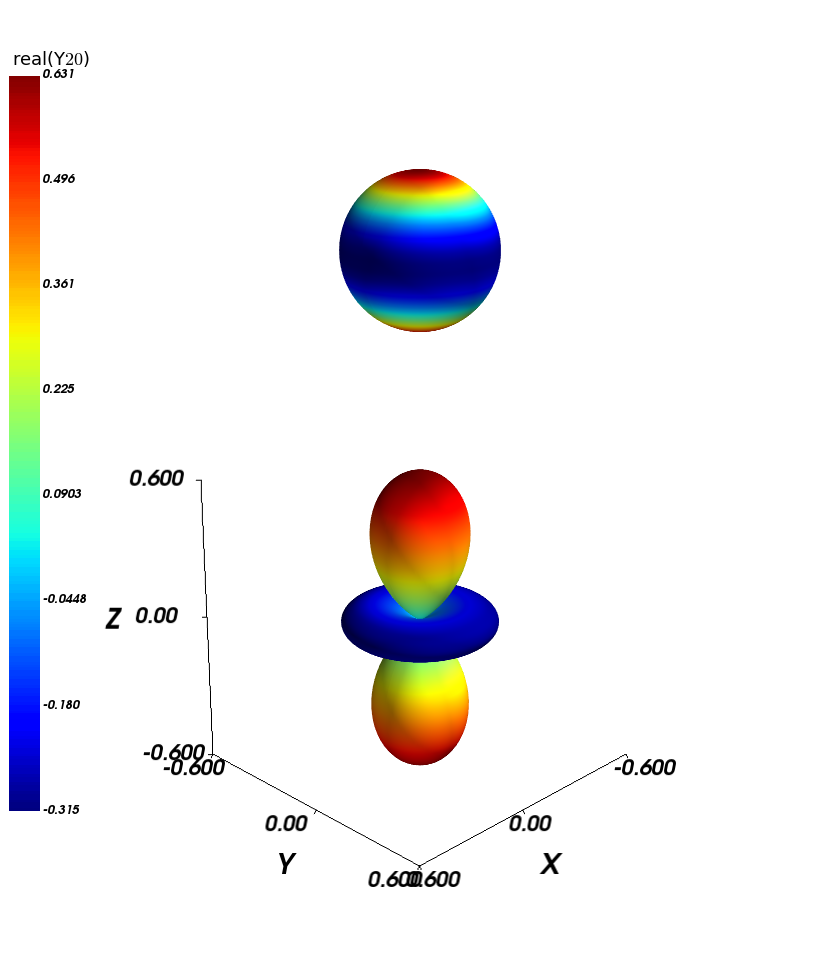
\includegraphics[height=0.17\textwidth]{Figures/y20.png} &
    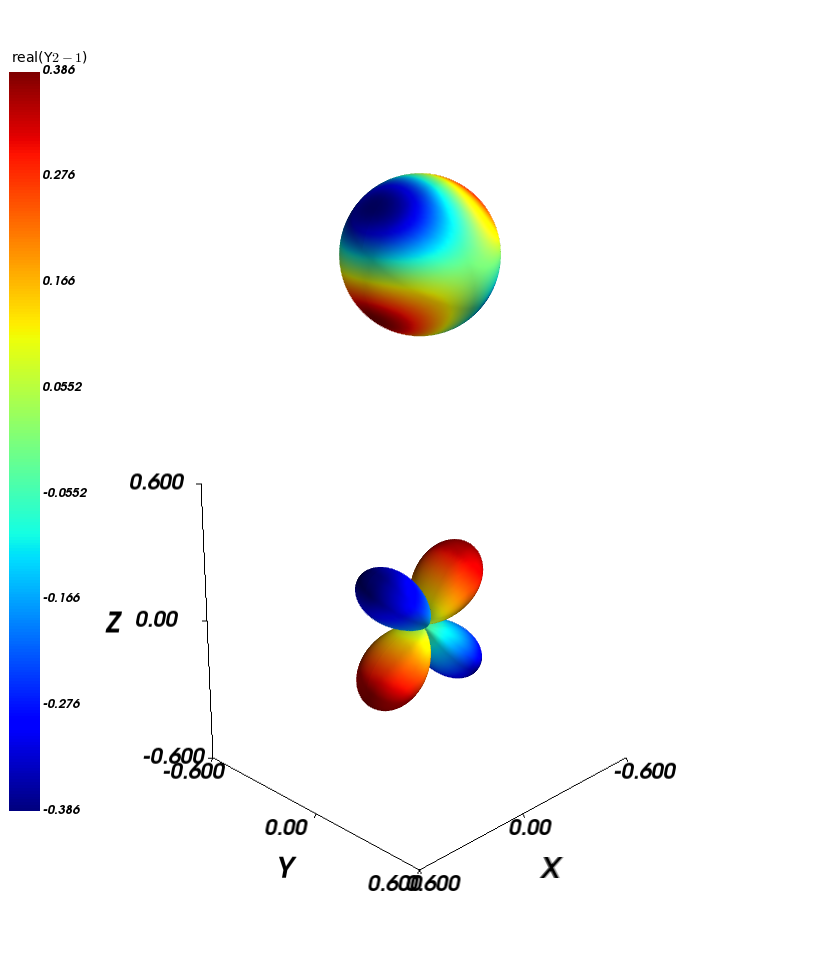
\includegraphics[height=0.17\textwidth]{Figures/y2-1.png} &
    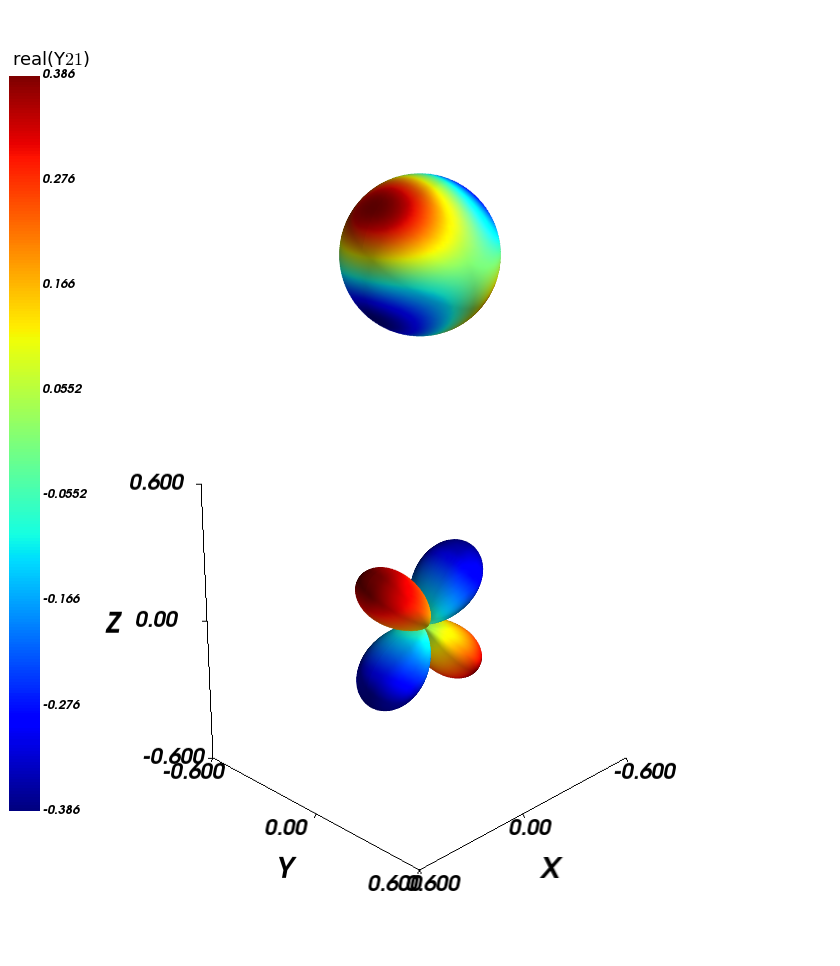
\includegraphics[height=0.17\textwidth]{Figures/y21.png} &
    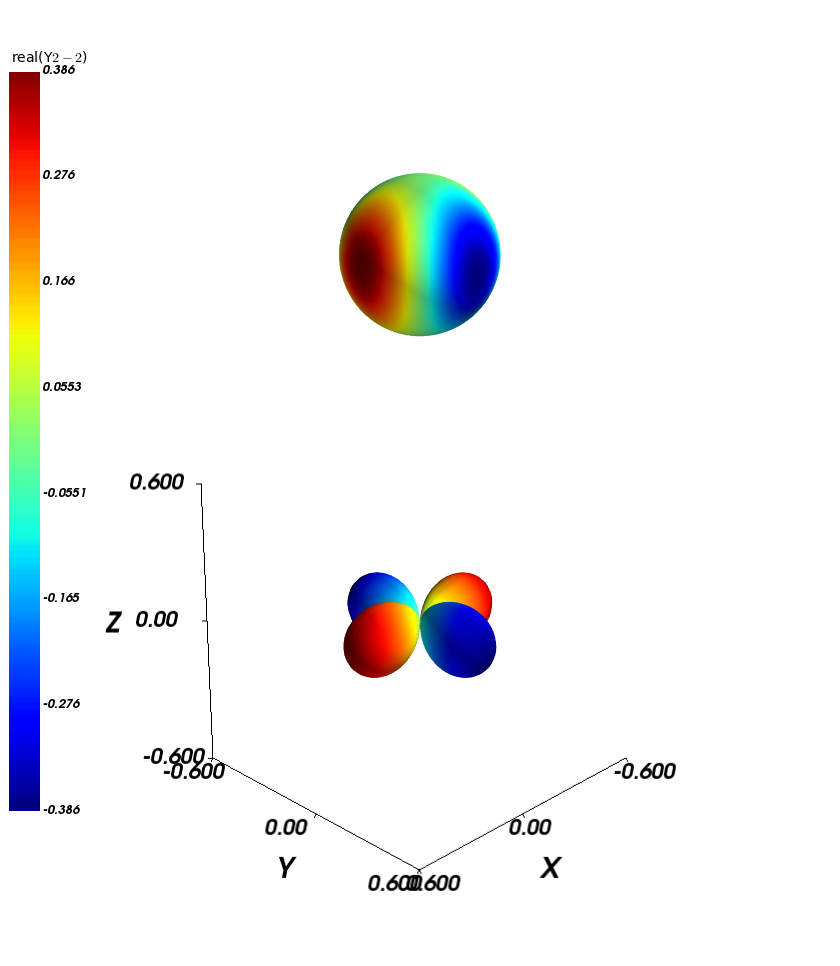
\includegraphics[height=0.17\textwidth]{Figures/y2-2.png} &
    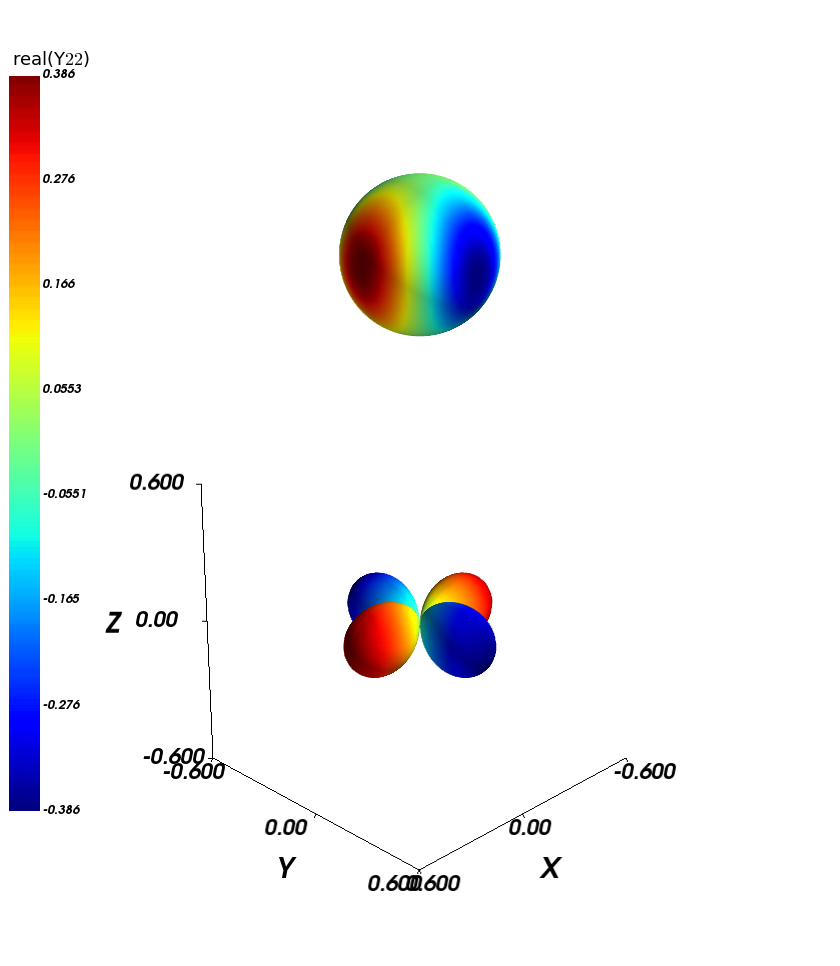
\includegraphics[height=0.17\textwidth]{Figures/y22.png} \\ \hline
    \hline
    \textbf{Imaginary} & m = 0 & m = -1 & m = 1 & m = -2 & m = 2 \\ \hline
    l = 0 & 
\includegraphics[height=0.17\textwidth]{Figures/y00_i.png} &&&& \\ \hline
    l = 1 && 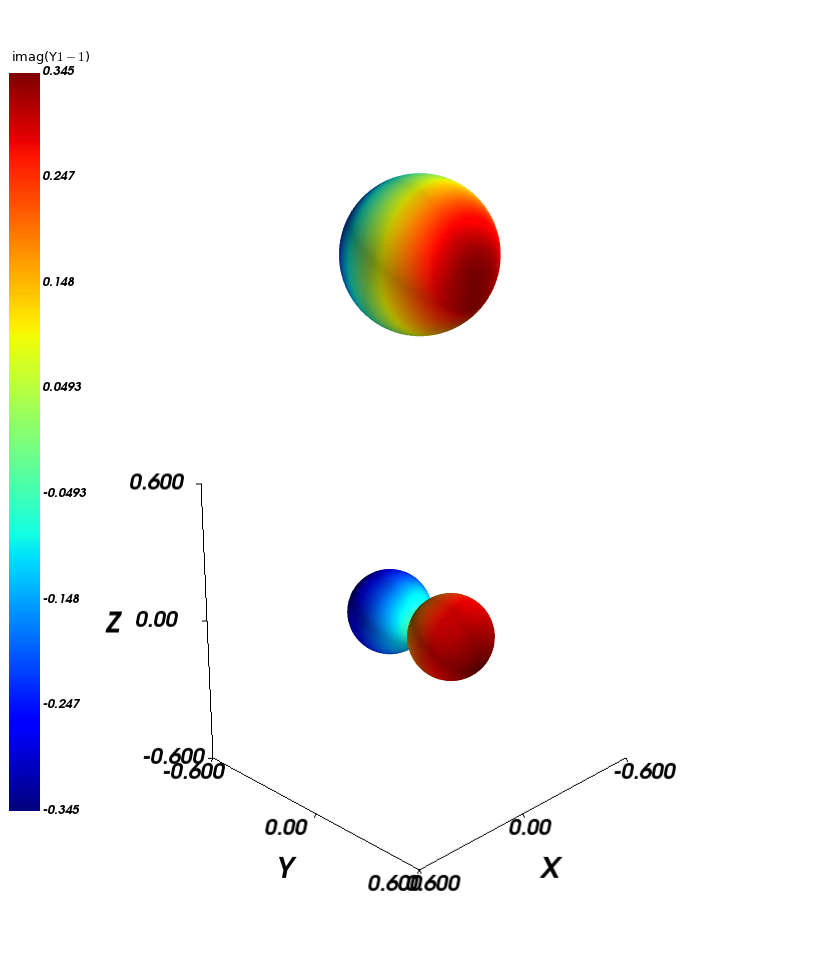
\includegraphics[height=0.17\textwidth]{Figures/y1-1_i.png} &
    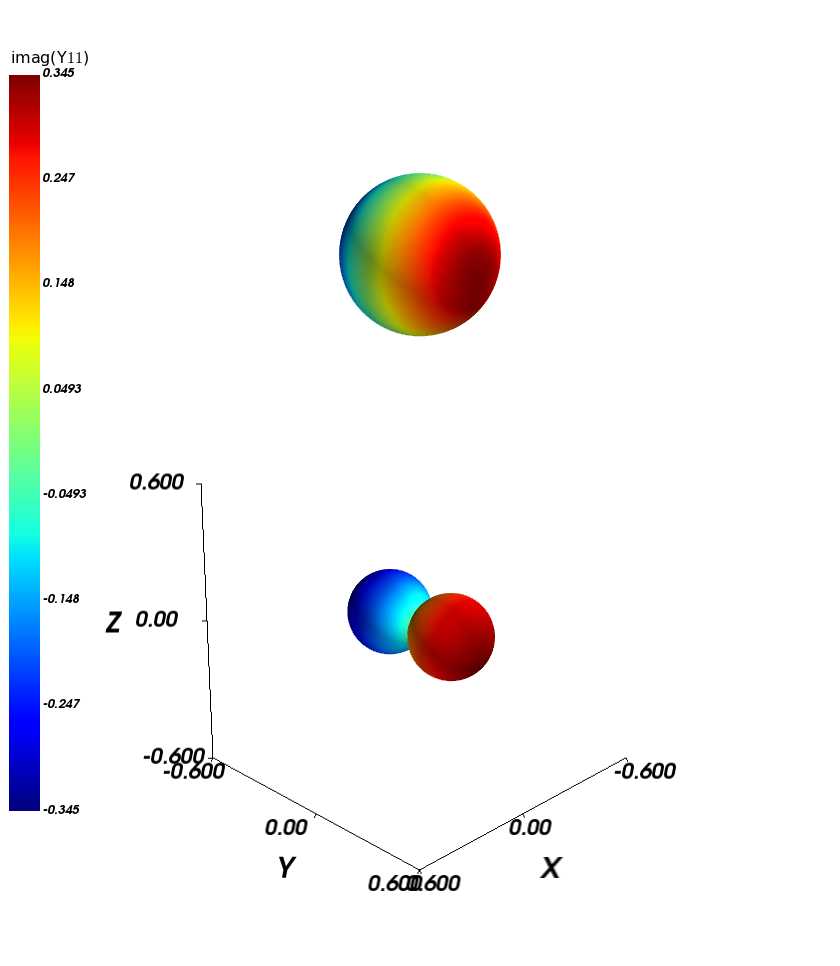
\includegraphics[height=0.17\textwidth]{Figures/y11_i.png}  && \\ \hline
    l = 2 && 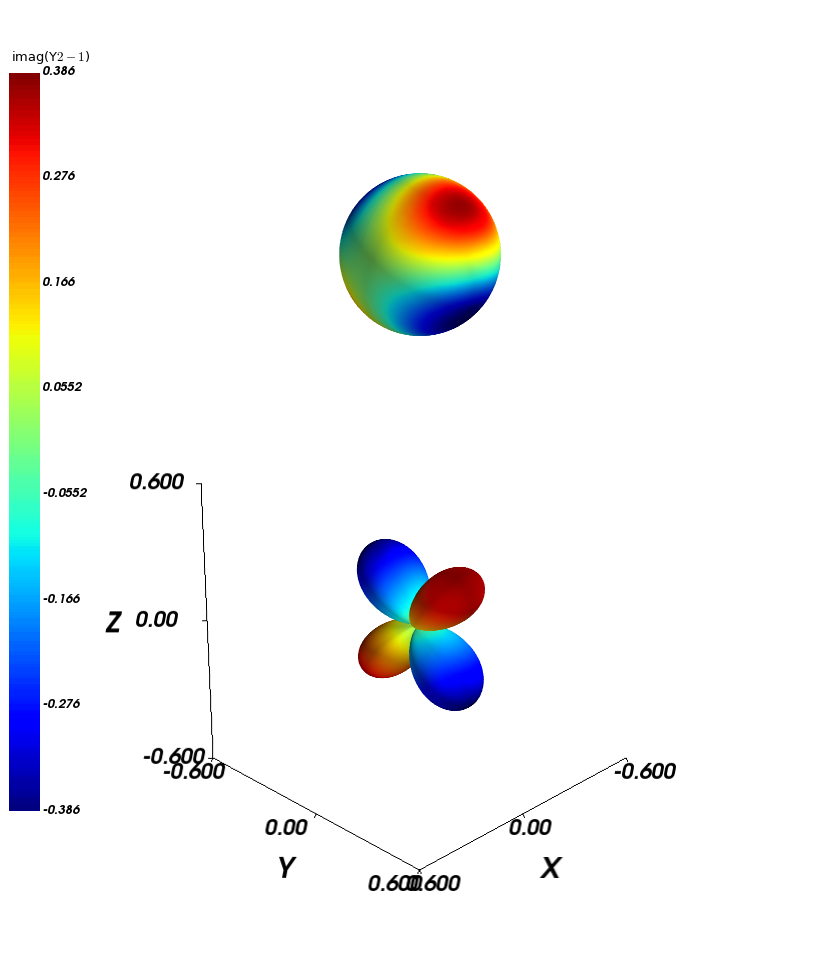
\includegraphics[height=0.17\textwidth]{Figures/y2-1_i.png} &
    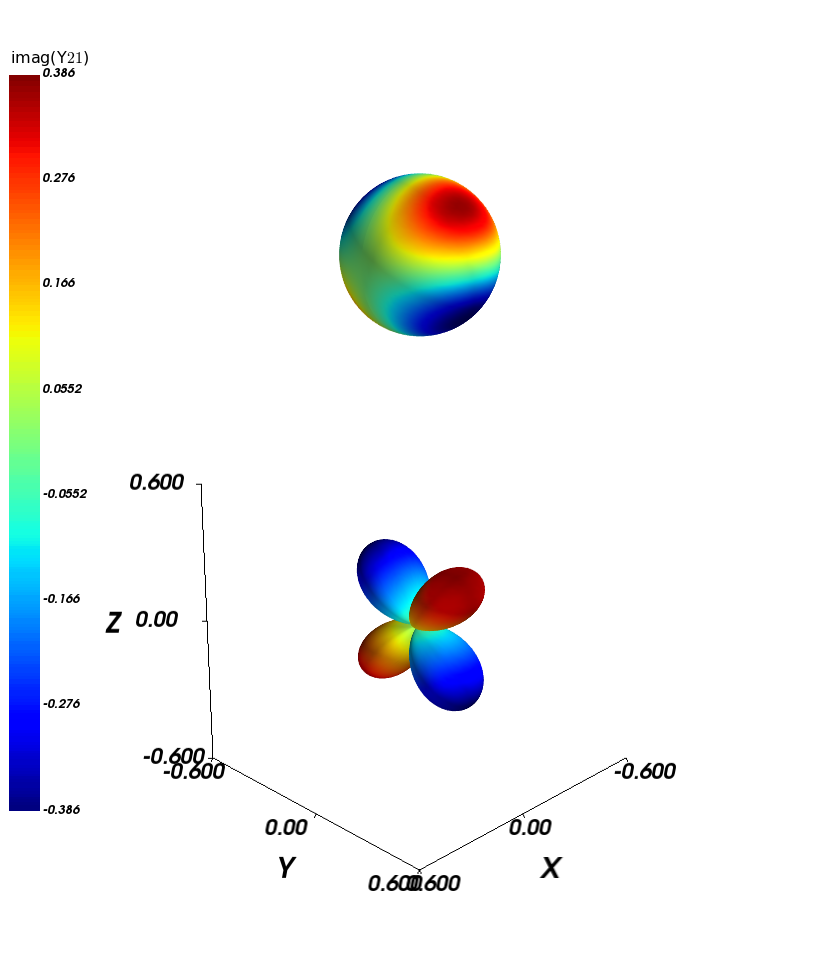
\includegraphics[height=0.17\textwidth]{Figures/y21_i.png} &
    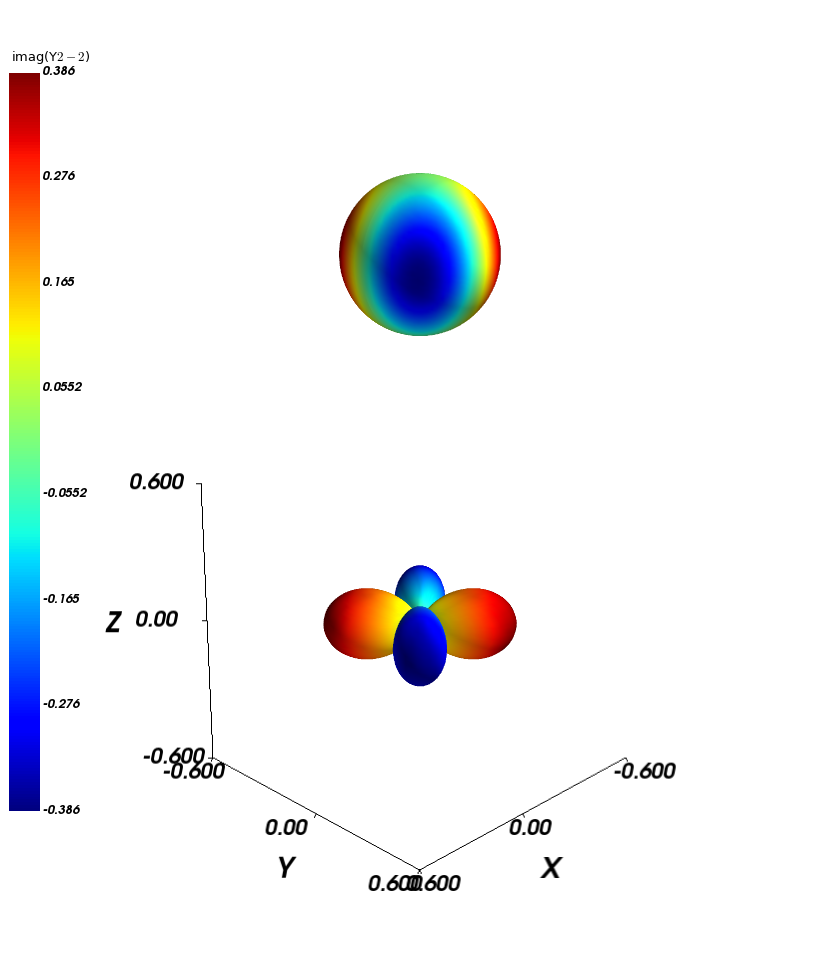
\includegraphics[height=0.17\textwidth]{Figures/y2-2_i.png} &
    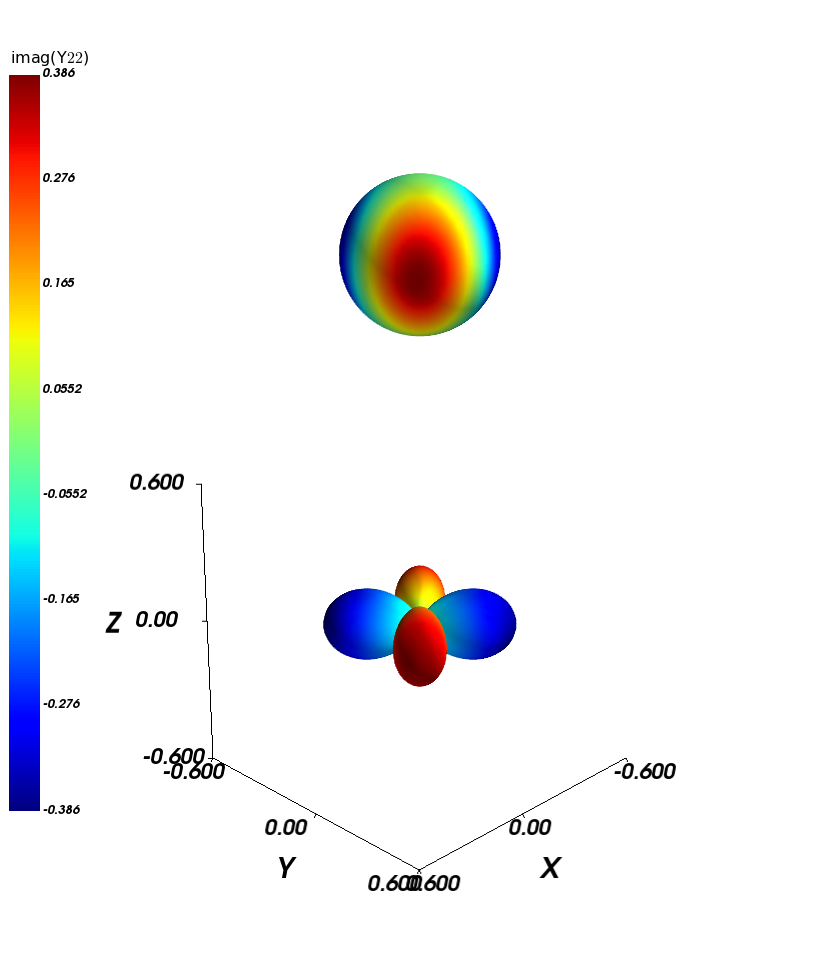
\includegraphics[height=0.17\textwidth]{Figures/y22_i.png} \\ \hline
    \end{tabular}
    \caption{Real and imaginary parts of the Spherical Harmonics for $l=0,1,2$ and $-l \leq m \leq l$. Notice that the imaginary parts are zero when $m=0$.}
    \label{fig1}
\end{figure}






\newpage
\begin{enumerate}[(b)]
    \item Now, we will approximate the external source. Using the S$_4$ quadrature to do the integrations and q$_e$ = 1 for all angles: use the equations for external source we developed in class, calculate the external source for $N = 0, 1, 2$.\\[-5pt]
\end{enumerate}


$\Rightarrow$ The expansion of external source can be written as follows
%
\begin{equation*}
  q^g_e(\vec{r}, \hat{\Omega}) = \sum_{l=0}^{N}\Bigl[Y^e_{l0}(\hat{\Omega})q^g_{l0}(\vec{r}) + \sum_{m=1}^{l}\bigr(Y^e_{lm}(\hat{\Omega})q^g_{lm}(\vec{r}) + Y^o_{lm}(\hat{\Omega})s^g_{lm}(\vec{r})\bigr)\Bigr]\:,
\end{equation*}

where $Y_{lm}$ are the spherical harmonics of order $l$ and degree $m$, $e$ and $o$ represent the even and odd moments, respectively, and the even and odd source moments are given by
%
\begin{align*}
  q^g_{lm} &= \int_{4\pi}Y^e_{lm}(\hat{\Omega})q^g_e(\hat{\Omega})\:d\hat{\Omega} = \int_{4\pi}Y^e_{lm}(\hat{\Omega})\:d\hat{\Omega}\:, \quad m\ge 0 \\
  s^g_{lm} &= \int_{4\pi}Y^o_{lm}(\hat{\Omega})q^g_e(\hat{\Omega})\:d\hat{\Omega} = \int_{4\pi}Y^o_{lm}(\hat{\Omega})\:d\hat{\Omega} \:, \quad m>0
\end{align*}

where
%
\begin{align*}
    Y_{lm}^e(\hat{\Omega}) = D_{lm}P_{lm}(\cos\theta)\cos(m\phi) \\
    Y_{lm}^o(\hat{\Omega}) = D_{lm}P_{lm}(\cos\theta)\sin(m\phi) \\
    D_{lm} = (-1)^m \sqrt{(2-\delta_{m0}) \frac{2l+1}{4\pi} \frac{(l-m)!}{(l+m)!}}
\end{align*}

Now we will need to evaluate these integrals for $l=0,1,2$ and $m=0\rightarrow l$. And we will us the S$_4$ quadrature to evaluate the integrals. The spherical harmonics are defined using $\theta$ and $\phi$ and the quadrature uses $\mu$, $\eta$, and $\xi$. Therefore we first need to convert from one to the other. In this treatment, $\mu$ is like $z$, $\eta$ is like $x$, and $\xi$ is like $y$. Therefore we have
\begin{align*}
    \theta &= \cos^{-1}(\mu) \\
    \phi &= \tan^{-1}\left(\frac{\xi}{\eta}\right)
\end{align*}


Next, we can use the quadrature code and the spherical harmonic code to evaluate all the integrals using S$_4$. In doing so (see the Python code below), we get the following results for the even components ($q_{lm}^g$) (accounting for the signs of $\mu$, $\eta$, and $\xi$ in the 8 octants):
%
\begin{align*}
  &q_{00}^g = \int_{4\pi}Y_{00}^e(\hat{\Omega})\:d\hat{\Omega} = \frac{4\pi}{24}\sum_{\textrm{8 octants}}Y_{00}^e(\mu_1,\eta_1,\xi_2) + Y_{00}^e(\mu_1,\eta_2,\xi_1) + Y_{00}^e(\mu_2,\eta_1,\xi_1) = 3.5449 \\
  &q_{10}^g =\int_{4\pi}Y_{10}^e(\hat{\Omega})\:d\hat{\Omega} = \frac{4\pi}{24}\sum_{\textrm{8 octants}}Y_{10}^e(\mu_1,\eta_1,\xi_2) + Y_{10}^e(\mu_1,\eta_2,\xi_1) + Y_{10}^e(\mu_2,\eta_1,\xi_1) \approx 0 \\
  &q_{11}^g =\int_{4\pi}Y_{11}^e(\hat{\Omega})\:d\hat{\Omega} = \frac{4\pi}{24}\sum_{\textrm{8 octants}}Y_{11}^e(\mu_1,\eta_1,\xi_2) + Y_{11}^e(\mu_1,\eta_2,\xi_1) + Y_{11}^e(\mu_2,\eta_1,\xi_1) \approx 0 \\
  &q_{20}^g =\int_{4\pi}Y_{20}^e(\hat{\Omega})\:d\hat{\Omega} = \frac{4\pi}{24}\sum_{\textrm{8 octants}}Y_{20}^e(\mu_1,\eta_1,\xi_2) + Y_{20}^e(\mu_1,\eta_2,\xi_1) + Y_{20}^e(\mu_2,\eta_1,\xi_1) \approx 0 \\
  &q_{21}^g =\int_{4\pi}Y_{21}^e(\hat{\Omega})\:d\hat{\Omega} = \frac{4\pi}{24}\sum_{\textrm{8 octants}}Y_{21}^e(\mu_1,\eta_1,\xi_2) + Y_{21}^e(\mu_1,\eta_2,\xi_1) + Y_{21}^e(\mu_2,\eta_1,\xi_1) \approx 0 \\
  &q_{22}^g =\int_{4\pi}Y_{22}^e(\hat{\Omega})\:d\hat{\Omega} = \frac{4\pi}{24}\sum_{\textrm{8 octants}}Y_{22}^e(\mu_1,\eta_1,\xi_2) + Y_{22}^e(\mu_1,\eta_2,\xi_1) + Y_{22}^e(\mu_2,\eta_1,\xi_1) \approx 0 \\
\end{align*}

Notice the factor of (1/24), this is because of the (4$\pi$/8) out in front being multiplied by the (1/3) weight for each quadrature point. I used the $\approx$ symbol, because the calculation gave very small answers in most cases ($\sim 10^{-16}$). Also note that there is no spatial dependence in the final results. For the odd components ($s_{lm}^g$), we get
%
\begin{align*}
  &s_{00}^g = \int_{4\pi}Y_{00}^o(\hat{\Omega})\:d\hat{\Omega} = \frac{4\pi}{24}\sum_{\textrm{8 octants}}Y_{00}^o(\mu_1,\eta_1,\xi_2) + Y_{00}^o(\mu_1,\eta_2,\xi_1) + Y_{00}^o(\mu_2,\eta_1,\xi_1) \approx 0 \\
  &s_{10}^g =\int_{4\pi}Y_{10}^o(\hat{\Omega})\:d\hat{\Omega} = \frac{4\pi}{24}\sum_{\textrm{8 octants}}Y_{10}^o(\mu_1,\eta_1,\xi_2) + Y_{10}^o(\mu_1,\eta_2,\xi_1) + Y_{10}^o(\mu_2,\eta_1,\xi_1) \approx 0 \\
  &s_{11}^g =\int_{4\pi}Y_{11}^o(\hat{\Omega})\:d\hat{\Omega} = \frac{4\pi}{24}\sum_{\textrm{8 octants}}Y_{11}^o(\mu_1,\eta_1,\xi_2) + Y_{11}^o(\mu_1,\eta_2,\xi_1) + Y_{11}^o(\mu_2,\eta_1,\xi_1) \approx 0 \\
  &s_{20}^g =\int_{4\pi}Y_{20}^o(\hat{\Omega})\:d\hat{\Omega} = \frac{4\pi}{24}\sum_{\textrm{8 octants}}Y_{20}^o(\mu_1,\eta_1,\xi_2) + Y_{20}^o(\mu_1,\eta_2,\xi_1) + Y_{20}^o(\mu_2,\eta_1,\xi_1) \approx 0 \\
  &s_{21}^g =\int_{4\pi}Y_{21}^o(\hat{\Omega})\:d\hat{\Omega} = \frac{4\pi}{24}\sum_{\textrm{8 octants}}Y_{21}^o(\mu_1,\eta_1,\xi_2) + Y_{21}^o(\mu_1,\eta_2,\xi_1) + Y_{21}^o(\mu_2,\eta_1,\xi_1) \approx 0 \\
  &s_{22}^g =\int_{4\pi}Y_{22}^o(\hat{\Omega})\:d\hat{\Omega} = \frac{4\pi}{24}\sum_{\textrm{8 octants}}Y_{22}^o(\mu_1,\eta_1,\xi_2) + Y_{22}^o(\mu_1,\eta_2,\xi_1) + Y_{22}^o(\mu_2,\eta_1,\xi_1) \approx 0 \\
\end{align*}

Again, all the calculations results in either zero or very small numbers. These results make sense we when analytically calculate the integrals, which is easy enough to check with Mathematica. And this makes our life easier because all of the terms are zero except for $q_{00}^g$. So, plugging these results back into our external source expansion, we get the following for $N=0,1,2$
%
\begin{align*}
    &N = 0 \quad \Rightarrow \quad q_e^g(\vec{r},\hat{\Omega}) = Y_{00}^e(\hat{\Omega}) q_{00}^g = \frac{3.5449}{2} \sqrt{\frac{1}{\pi}}\\
    &N = 1 \quad \Rightarrow \quad q_e^g(\vec{r},\hat{\Omega}) = Y_{00}^e(\hat{\Omega}) q_{00}^g = \frac{3.5449}{2} \sqrt{\frac{1}{\pi}}\\
    &N = 2 \quad \Rightarrow \quad q_e^g(\vec{r},\hat{\Omega}) = Y_{00}^e(\hat{\Omega}) q_{00}^g = \frac{3.5449}{2} \sqrt{\frac{1}{\pi}}
\end{align*}

We see that this is just a constant value over all space and angle. This makes sense because we used $q_e = 1$, which is to say the source strength is constant and uniform over all space and angle, so it is reasonable that the spherical harmonic expansion of the source will also be constant in space and angle.\\

\lstinputlisting[language=Python]{../p4/b/p4b.py}


\begin{lstlisting}[numbers=none]
OUTPUT:

l =  0, m = 0, qlm = 3.54490770181
l =  0, m = 0, slm = 0.0
l =  1, m = 0, qlm = 2.83912495738e-13
l =  1, m = 0, slm = 0.0
l =  1, m = 1, qlm = 2.90655708167e-16
l =  1, m = 1, slm = 5.81311416335e-17
l =  2, m = 0, qlm = 2.18032173099e-07
l =  2, m = 0, slm = 0.0
l =  2, m = 1, qlm = -1.16262283267e-16
l =  2, m = 1, slm = -2.32524566534e-16
l =  2, m = 2, qlm = -2.77665249661e-16
l =  2, m = 2, slm = 0.0
\end{lstlisting}






% - - - - - - - - - - - - - - - - - - - - - - - - - - - - - - - - - - - - - - - - - -
\newpage
\noindent \textbf{Problem 5}\\
What are the major nuclear data libraries and which countries manage them?\\[5pt]

$\Rightarrow$ The three major nuclear data libraries are the Evaluated Nuclear Data File (ENDF), Joint Evaluated Fission and Fusion File (JEFF), and Japanese Evaluated Nuclear Data Library (JENDL). ENDF is managed by a Canadian and USA cross section working group consisting of national laboratories, universities, and industry. JEFF is managed by the Nuclear Energy Agency under the Organization for Economic Cooperation and Development (OECD) - which previoulsy consisted of only European member states until 1961. JENDL is managed by the Nuclear Data Center within the Japan Atomic Energy Agency (JAEA) in Japan.\\

There are also other data libraries such as the Experimental Nuclear Reaction Data (EXFOR) managed by the IAEA (comprised of multiple countries including the US, Russia, Japan, Austria, France, etc.), as well as modeling codes used to produce data for the libraries (such as EMPIRE and TALYS) and codes to convert the libraries into other useable formats (such as RIPL), all primarily managed by the nuclear data group at the IAEA. 




\end{document}
